\documentclass[11pt,a4paper]{ctexart}
% Shared preamble for the assignment reports. Use with:
%   \documentclass[11pt,a4paper]{ctexart}  (XeLaTeX)
%   % Shared preamble for the assignment reports. Use with:
%   \documentclass[11pt,a4paper]{ctexart}  (XeLaTeX)
%   % Shared preamble for the assignment reports. Use with:
%   \documentclass[11pt,a4paper]{ctexart}  (XeLaTeX)
%   \input{../common/preamble.tex}
\usepackage[margin=2.3cm]{geometry}
\setmainfont{texgyretermes}[Extension=.otf,UprightFont=*-regular,BoldFont=*-bold,ItalicFont=*-italic,BoldItalicFont=*-bolditalic]
\setsansfont{texgyreheros}[Extension=.otf,UprightFont=*-regular,BoldFont=*-bold,ItalicFont=*-italic,BoldItalicFont=*-bolditalic]
\setmonofont{texgyrecursor}[Extension=.otf,UprightFont=*-regular,BoldFont=*-bold,ItalicFont=*-italic,BoldItalicFont=*-bolditalic]
\usepackage{amsmath,amssymb,mathtools,bm}
\usepackage{graphicx}
\usepackage{booktabs,multirow,makecell,array,tabularx}
\usepackage[table]{xcolor}
\usepackage[most]{tcolorbox}
\usepackage{enumitem}
\usepackage{listings}
\usepackage{subcaption}
\usepackage{siunitx}
\usepackage[hidelinks]{hyperref}
\usepackage[nameinlink,noabbrev]{cleveref}
\usepackage{float}

\setlength{\emergencystretch}{3em}
\linespread{1.15}
\setlist{leftmargin=*,itemsep=2pt,topsep=3pt}
\graphicspath{{figures/}}

\crefname{figure}{图}{图}
\crefname{table}{表}{表}
\crefname{section}{第}{第}
\creflabelformat{section}{#2#1#3 节}
\crefname{equation}{式}{式}
\crefformat{equation}{式~(#2#1#3)}

\lstset{basicstyle=\ttfamily\footnotesize,columns=fullflexible,breaklines=true,frame=single,
  framerule=0.3pt,rulecolor=\color{black!40},backgroundcolor=\color{black!3},
  keywordstyle=\color{blue!60!black}\bfseries,commentstyle=\color{green!40!black},
  numbers=left,numberstyle=\tiny\color{black!50},xleftmargin=1.5em}

% Interview boxes: question, model answer, common wrong answer.
\newtcolorbox{iqbox}[1]{enhanced,breakable,colback=blue!3,colframe=blue!45!black,boxrule=0.5pt,arc=1.5pt,
  left=4pt,right=4pt,top=3pt,bottom=3pt,fonttitle=\bfseries\small,title={面试追问：#1}}
\newtcolorbox{findingbox}[1][]{enhanced,breakable,colback=green!3,colframe=green!40!black,boxrule=0.5pt,arc=1.5pt,
  left=4pt,right=4pt,top=3pt,bottom=3pt,fonttitle=\bfseries\small,title={结论#1}}
\newtcolorbox{caveatbox}{enhanced,breakable,colback=orange!4,colframe=orange!60!black,boxrule=0.5pt,arc=1.5pt,
  left=4pt,right=4pt,top=3pt,bottom=3pt,fonttitle=\bfseries\small,title={不能推出的结论}}

\newcommand{\authorline}{ShaneLiu04\thanks{GitHub: \url{https://github.com/ShaneLiu04}。代码与原始指标见 edge-deploy 仓库各 lab 的 \texttt{artifacts/raw/}。本文基于公开课程材料独立完成，与课程团队无隶属关系。}}

\usepackage[margin=2.3cm]{geometry}
\setmainfont{texgyretermes}[Extension=.otf,UprightFont=*-regular,BoldFont=*-bold,ItalicFont=*-italic,BoldItalicFont=*-bolditalic]
\setsansfont{texgyreheros}[Extension=.otf,UprightFont=*-regular,BoldFont=*-bold,ItalicFont=*-italic,BoldItalicFont=*-bolditalic]
\setmonofont{texgyrecursor}[Extension=.otf,UprightFont=*-regular,BoldFont=*-bold,ItalicFont=*-italic,BoldItalicFont=*-bolditalic]
\usepackage{amsmath,amssymb,mathtools,bm}
\usepackage{graphicx}
\usepackage{booktabs,multirow,makecell,array,tabularx}
\usepackage[table]{xcolor}
\usepackage[most]{tcolorbox}
\usepackage{enumitem}
\usepackage{listings}
\usepackage{subcaption}
\usepackage{siunitx}
\usepackage[hidelinks]{hyperref}
\usepackage[nameinlink,noabbrev]{cleveref}
\usepackage{float}

\setlength{\emergencystretch}{3em}
\linespread{1.15}
\setlist{leftmargin=*,itemsep=2pt,topsep=3pt}
\graphicspath{{figures/}}

\crefname{figure}{图}{图}
\crefname{table}{表}{表}
\crefname{section}{第}{第}
\creflabelformat{section}{#2#1#3 节}
\crefname{equation}{式}{式}
\crefformat{equation}{式~(#2#1#3)}

\lstset{basicstyle=\ttfamily\footnotesize,columns=fullflexible,breaklines=true,frame=single,
  framerule=0.3pt,rulecolor=\color{black!40},backgroundcolor=\color{black!3},
  keywordstyle=\color{blue!60!black}\bfseries,commentstyle=\color{green!40!black},
  numbers=left,numberstyle=\tiny\color{black!50},xleftmargin=1.5em}

% Interview boxes: question, model answer, common wrong answer.
\newtcolorbox{iqbox}[1]{enhanced,breakable,colback=blue!3,colframe=blue!45!black,boxrule=0.5pt,arc=1.5pt,
  left=4pt,right=4pt,top=3pt,bottom=3pt,fonttitle=\bfseries\small,title={面试追问：#1}}
\newtcolorbox{findingbox}[1][]{enhanced,breakable,colback=green!3,colframe=green!40!black,boxrule=0.5pt,arc=1.5pt,
  left=4pt,right=4pt,top=3pt,bottom=3pt,fonttitle=\bfseries\small,title={结论#1}}
\newtcolorbox{caveatbox}{enhanced,breakable,colback=orange!4,colframe=orange!60!black,boxrule=0.5pt,arc=1.5pt,
  left=4pt,right=4pt,top=3pt,bottom=3pt,fonttitle=\bfseries\small,title={不能推出的结论}}

\newcommand{\authorline}{ShaneLiu04\thanks{GitHub: \url{https://github.com/ShaneLiu04}。代码与原始指标见 edge-deploy 仓库各 lab 的 \texttt{artifacts/raw/}。本文基于公开课程材料独立完成，与课程团队无隶属关系。}}

\usepackage[margin=2.3cm]{geometry}
\setmainfont{texgyretermes}[Extension=.otf,UprightFont=*-regular,BoldFont=*-bold,ItalicFont=*-italic,BoldItalicFont=*-bolditalic]
\setsansfont{texgyreheros}[Extension=.otf,UprightFont=*-regular,BoldFont=*-bold,ItalicFont=*-italic,BoldItalicFont=*-bolditalic]
\setmonofont{texgyrecursor}[Extension=.otf,UprightFont=*-regular,BoldFont=*-bold,ItalicFont=*-italic,BoldItalicFont=*-bolditalic]
\usepackage{amsmath,amssymb,mathtools,bm}
\usepackage{graphicx}
\usepackage{booktabs,multirow,makecell,array,tabularx}
\usepackage[table]{xcolor}
\usepackage[most]{tcolorbox}
\usepackage{enumitem}
\usepackage{listings}
\usepackage{subcaption}
\usepackage{siunitx}
\usepackage[hidelinks]{hyperref}
\usepackage[nameinlink,noabbrev]{cleveref}
\usepackage{float}

\setlength{\emergencystretch}{3em}
\linespread{1.15}
\setlist{leftmargin=*,itemsep=2pt,topsep=3pt}
\graphicspath{{figures/}}

\crefname{figure}{图}{图}
\crefname{table}{表}{表}
\crefname{section}{第}{第}
\creflabelformat{section}{#2#1#3 节}
\crefname{equation}{式}{式}
\crefformat{equation}{式~(#2#1#3)}

\lstset{basicstyle=\ttfamily\footnotesize,columns=fullflexible,breaklines=true,frame=single,
  framerule=0.3pt,rulecolor=\color{black!40},backgroundcolor=\color{black!3},
  keywordstyle=\color{blue!60!black}\bfseries,commentstyle=\color{green!40!black},
  numbers=left,numberstyle=\tiny\color{black!50},xleftmargin=1.5em}

% Interview boxes: question, model answer, common wrong answer.
\newtcolorbox{iqbox}[1]{enhanced,breakable,colback=blue!3,colframe=blue!45!black,boxrule=0.5pt,arc=1.5pt,
  left=4pt,right=4pt,top=3pt,bottom=3pt,fonttitle=\bfseries\small,title={面试追问：#1}}
\newtcolorbox{findingbox}[1][]{enhanced,breakable,colback=green!3,colframe=green!40!black,boxrule=0.5pt,arc=1.5pt,
  left=4pt,right=4pt,top=3pt,bottom=3pt,fonttitle=\bfseries\small,title={结论#1}}
\newtcolorbox{caveatbox}{enhanced,breakable,colback=orange!4,colframe=orange!60!black,boxrule=0.5pt,arc=1.5pt,
  left=4pt,right=4pt,top=3pt,bottom=3pt,fonttitle=\bfseries\small,title={不能推出的结论}}

\newcommand{\authorline}{ShaneLiu04\thanks{GitHub: \url{https://github.com/ShaneLiu04}。代码与原始指标见 edge-deploy 仓库各 lab 的 \texttt{artifacts/raw/}。本文基于公开课程材料独立完成，与课程团队无隶属关系。}}

\graphicspath{{../../solutions/edge-runtime/q4-gemv/artifacts/figures/}}

\title{q4-gemv 实验报告：llama.cpp 块量化的 GEMV、\\解码带宽上界与 GPT-2 困惑度，CPU 指令受限而 GPU 带宽受限}
\author{\authorline}
\date{2026 年 11 月}

\begin{document}
\maketitle

\begin{abstract}
端侧 LLM 解码每生成一个 token 要把全部权重读一遍，batch 1 的 GEMV 被带宽限住；llama.cpp 的 Q8\_0 / Q4\_0 / Q4\_1 把每 32 个权重和一个 fp16 scale 打成一块来减字节。
本报告是 q4-gemv lab 的专题报告：用 NumPy 实现三种块格式并与 gguf 参考逐字节一致，用 C++ 写 9 种 GEMV（fp32、fp16、Q8 / Q4 的浮点融合、先反量化、VNNI 整数点积及其 4 累加器版），
在 4 核 Ice Lake 虚拟机和 Xeon 8470Q 服务器上计时；不依赖 transformers 实现 GPT-2 前向，在 wikitext-2 全部 280 个窗口上测困惑度；
再用 Triton 在 RTX 6000D 上实现融合反量化 GEMV，并把 Qwen2.5-7B 的 196 个层内 Linear 加 lm\_head 的时间相加，预测整模型解码速度。

主要结论：
（a）融合是前提：Q4\_0 先反量化再点积 4541 µs，与 fp32 的 4763 µs 差不多；整数点积（Q4 × Q8 VNNI）单线程 1034 µs，比 fp32 快 4.6 倍，但字节少 7.1 倍，实际只有 9.1 GB/s；
（b）CPU 上 Q4 是指令受限的：本机单线程 Q8 × Q8 与 Q4 × Q8 持平（1009 对 1034 µs），4 线程 Q8 反超（275 对 311 µs）；服务器上 1、4、16 线程两者都相差不到 6\%；
4 个独立累加器只让 Q4 快 4\%，瓶颈是每块的指令吞吐而不是 FMA 依赖链；
（c）质量：GPT-2 124M 的困惑度 fp32 29.951、Q8\_0 29.953、Q4\_0 31.88、Q4\_1 32.15；Q4\_1 的层平均 SQNR 更高（21.96 对 21.03 dB）困惑度却更差；Q8 与 Q4 的 SQNR 差 24.04 dB，接近每 bit 6.02 dB 的理论值；
（d）GPU 上融合反量化 GEMV 只剩搬字节：lm\_head 上 Triton Q4\_0 231 µs、1327 GB/s（实测读带宽的 99.5\%），比 cuBLAS fp16 快 3.63 倍，恰好接近 16 / 4.5 的字节比；
（e）下发开销决定小层：eager 时每次 Triton 调用约 22 µs，Q4 解码只预测到 176 tok/s；CUDA graph 后预测 fp16 92、Q8\_0 163、Q4\_0 284 tok/s；
（f）llama-cpp-7b 报告在同一张卡上端到端测得 87.9 / 152.8 / 250.7 tok/s，比预测多一个与格式无关的常数 0.41--0.47 ms/token：层时间相加的模型在结构上是对的。
\end{abstract}

\tableofcontents
\newpage

\section{这个实验要回答什么}\label{sec:questions}

端侧推理面试里最常见的一句话是“4 bit 量化让解码快 4 倍”。这句话里藏着三个需要分开验证的假设：
解码时间正比于权重字节；4 bit 格式的字节真的是 fp16 的 1/4；内核能把省下的字节兑现成时间。
q4-gemv 把这三件事拆开来测。具体地，本报告要回答五个问题：

\begin{enumerate}[label=Q\arabic*.]
  \item \textbf{块格式到底多少字节？}Q8\_0、Q4\_0、Q4\_1 每 32 个权重带一个或两个 fp16 参数，bit/权重是 8.5、4.5、5.0，而不是 8 和 4。
        自己写的打包器能否与 llama.cpp~\cite{llamacpp} 的 gguf 参考逐字节一致？（\cref{sec:formats,sec:byteexact}）
  \item \textbf{解码速度的天花板在哪里？}tok/s $\le$ 带宽 / 权重字节（E25）。Pi 5、Orin Nano 和本机分别是多少？（\cref{sec:bound,sec:res-bound}）
  \item \textbf{CPU 内核能不能碰到天花板？}先反量化、浮点融合、整数点积三种 Q4 内核分别拿到字节比的多少？Q4 读的字节只有 Q8 的一半，为什么不更快？（\cref{sec:res-cpu,sec:server}）
  \item \textbf{精度代价多大？}GPT-2~\cite{gpt2} 124M 上 Q8\_0 / Q4\_0 / Q4\_1 的困惑度，与 mlsys-infra 的 GPTQ~\cite{gptq} / RTN 在同一协议下怎么比？SQNR 能否预测困惑度？（\cref{sec:res-ppl}）
  \item \textbf{换成 GPU 结论还成立吗？}同样的块格式在 RTX 6000D 上能否打满带宽？只把 Linear 时间相加的解码预测，离端到端的 llama.cpp 有多远？（\cref{sec:gpu}）
\end{enumerate}

与仓库里其他报告的关系：edge-runtime-server 报告把包括本 lab 在内的 6 个 lab 搬到 Xeon 8470Q 与 RTX 6000D 上重跑，只用一节概述 Q4 GEMV；
llama-cpp-7b 报告用 llama.cpp 跑完整的 Qwen2.5-7B，端到端检验了本 lab 的 GPU 解码预测。本报告是这个 lab 的完整记录，
所有数字都来自 lab 的 \texttt{README.md} 与 \nolinkurl{artifacts/raw/}（\texttt{summary.json}、\texttt{gemv\_bench.csv}、\texttt{decode\_bound.csv}、\texttt{gpt2\_ppl.csv}、
\texttt{gpt2\_layer\_sqnr.csv}、\nolinkurl{gpu/*.csv}、\nolinkurl{xeon8470q/*}），引用其他报告的数字会注明出处。公式编号沿用 \nolinkurl{interview/FORMULAS.md} 的 E 编号。

\section{设置}\label{sec:setup}

\begin{table}[H]
\centering\small
\caption{三个平台}\label{tab:hosts}
\begin{tabularx}{\linewidth}{>{\raggedright\arraybackslash}p{1.6cm} >{\raggedright\arraybackslash}X >{\raggedright\arraybackslash}X >{\raggedright\arraybackslash}X}
\toprule
 & 本机（主平台） & 服务器 CPU & 服务器 GPU \\
\midrule
型号 & Ice Lake-SP 服务器虚拟机 & 2 × Xeon Platinum 8470Q（Sapphire Rapids） & NVIDIA RTX 6000D（sm\_120） \\
规模 & 4 物理核 & 绑 NUMA1 的 16 个物理核，每插槽 105 MB L3 & 156 SM，112 MB L2，84 GB GDDR7（448 bit） \\
ISA / 单元 & AVX-512、VNNI & AVX-512、VNNI、AMX-INT8 & CUDA core；Tensor Core 只用于 W4A16 GEMM \\
实测屋顶 & 1 线程 DRAM 读 13.4 GB/s，fp32 154.9 GFLOP/s，int8 396.1 GOP/s；4 线程 48.4 GB/s、596.6 / 1492.7 & 1 线程 DRAM 读 17.5 GB/s，16 线程 193.5 GB/s（host-roofline） & 4 GB 顺序读 1333 GB/s，拷贝 1280 GB/s（理论 1398） \\
软件 & MinGW g++ 13.2，Windows & GCC 11.4，Linux 容器 & torch 2.8.0+cu128，Triton 3.4.0 \\
\bottomrule
\end{tabularx}
\end{table}

本机屋顶~\cite{roofline}数字来自 FORMULAS.md 开头的主机描述（host-roofline lab 实测），服务器屋顶来自 edge-runtime-server 报告的平台表与 host-roofline 的 xeon8470q 结果。

\begin{table}[H]
\centering\small
\caption{测量协议}\label{tab:protocol}
\begin{tabularx}{\linewidth}{>{\raggedright\arraybackslash}p{2.2cm} >{\raggedright\arraybackslash}X}
\toprule
CPU 形状 & GPT-2 MLP（\texttt{gpt2\_mlp\_768x3072}，3072 行 × 768 列）、Llama-1B attention（$2048^2$）与 MLP（8192×2048）、Llama-7B attention（$4096^2$）；服务器上加 Llama-7B MLP（11008×4096，fp32 180 MB） \\
CPU 权重 & 合成：$\mathcal{N}(0, 0.02^2)$，每 977 个元素放大 8 倍作离群值，“像训练过的 LLM 权重”；激活 $x_c = \sin(0.37c) + 0.1\cos(1.3c)$ \\
CPU 计时 & 每个形状 × 方法 3 次预热，15 次重复取中位数；所有方法在同一次运行里计时；本机 1 / 4 线程，服务器 1 / 2 / 4 / 8 / 16 线程（\texttt{EDGE\_THREADS}），按行切分给线程 \\
带宽口径 & “GB/s” = 该格式的权重字节 ÷ 中位时间（fp32 4 B、fp16 2 B、Q8\_0 34/32 B、Q4\_0 18/32 B 每权重），不计激活与输出 \\
GPU 形状 & Llama-7B $4096^2$、11008×4096；Qwen2.5-7B 的 q/o 3584×3584、k/v 512×3584、gate/up 18944×3584、down 3584×18944、lm\_head 152064×3584 \\
GPU 计时 & CUDA event；“L2 冷”= 轮换足够多份权重拷贝使总工作集 $\ge 4$ GB（远超 112 MB L2），“热”= 同一份权重反复调用；eager 与 CUDA graph 两种下发各测一次 \\
困惑度 & wikitext-2 raw test，空行连接，280 个不重叠的 1024 token 窗口（286{,}440 个预测 token）；量化全部 48 个 Linear，lm\_head 与 wte 共享、保持 fp32 \\
\bottomrule
\end{tabularx}
\end{table}

两台 CPU 都没有硬件性能计数器权限，GPU 上 \texttt{ncu} 报 \texttt{ERR\_NVGPUCTRPERM}。本报告里所有“带宽受限 / 指令受限”的判断都来自“墙钟时间 ÷ 字节数”与实测屋顶的比较，以及控制变量的对照实验（例如 4 累加器版），没有事务计数佐证。
服务器 CPU 实验用 \texttt{taskset} 绑在 NUMA1 的物理核上，容器的 cgroup 只有 22 个 CPU 的配额，宿主上还有其他租户；16 线程的个别点可能被限流，后文只采用单调、可重复的结论。

\section{方法与推导}\label{sec:method}

\subsection{三种块格式}\label{sec:formats}

\begin{table}[H]
\centering\small
\caption{llama.cpp 的三种基础块格式（\texttt{ggml-common.h}；\texttt{code/blockq/pack.py}）}\label{tab:formats}
\begin{tabularx}{\linewidth}{l>{\raggedright\arraybackslash}p{4.3cm}rr>{\raggedright\arraybackslash}X}
\toprule
格式 & 块结构 & 块字节 & bit/权重 & 反量化 \\
\midrule
Q8\_0 & \texttt{\{fp16 d; int8 qs[32]\}} & 34 & 8.5 & $w = d\,q$，$d = \max|x| / 127$ \\
Q4\_0 & \texttt{\{fp16 d; uint8 qs[16]\}} & 18 & 4.5 & $w = d\,(q - 8)$，$d = x_{\text{absmax}} / (-8)$ \\
Q4\_1 & \texttt{\{fp16 d; fp16 m;} \texttt{uint8 qs[16]\}} & 20 & 5.0 & $w = d\,q + m$，$d = (\max - \min)/15$，$m = \min$ \\
\bottomrule
\end{tabularx}
\end{table}

\paragraph{E25 的前半：bit/权重。}每块 32 个权重，
\begin{equation}
\text{bpw} = \frac{\text{块字节} \times 8}{32}, \qquad \text{Q8\_0}: \tfrac{34 \times 8}{32} = 8.5,\quad \text{Q4\_0}: 4.5,\quad \text{Q4\_1}: 5.0 .
\label{eq:bpw}
\end{equation}
一个 fp16 scale 摊到 32 个权重上是 0.5 bit；若分组改成 128（mlsys-infra 的 g128），开销降到 0.125 bit。常见错答是“4 bit 是 fp16 的 1/4”：真实的字节比是 $4.5/16 = 0.281$，即 fp16 / Q4\_0 = 3.56 倍，fp32 / Q4\_0 = 7.1 倍。

\paragraph{Q4\_0 的符号技巧。}Q4\_0 的 $d$ 不是 $\max|x|/7$ 或 $/8$，而是 $x_{\text{absmax}}/(-8)$，其中 $x_{\text{absmax}}$ 保留最大幅值元素的\emph{符号}。量化公式（ggml 参考实现）是
\begin{equation}
q_j = \min\bigl(15,\ \operatorname{trunc}(x_j / d + 8.5)\bigr).
\label{eq:q40}
\end{equation}
最大幅值元素满足 $x/d = -8$，$q = \operatorname{trunc}(0.5) = 0$，反量化回 $-8d = x_{\text{absmax}}$，\emph{精确无误差}；4 bit 的 16 个级 $\{-8,\dots,7\}$ 不对称，
多出来的那一级落在离群值所在的一侧，另一侧最多到 $7d$。测试 \texttt{test\_q4\_0\_largest\_element\_is\_exact} 构造 $w_5 = -0.8$、$w_6 = 0.3$，检查 $w_5$ 回到 $-0.8$（相对容差 $10^{-3}$，只留给 fp16 存 $d$ 的舍入），$w_6$ 的误差不超过半个步长。
Q4\_1 是非对称格式：16 级铺满 $[\min, \max]$，两个端点都在网格上，但零点不一定精确。

\paragraph{半字节排布。}Q4\_0 / Q4\_1 的第 $j$ 个字节低 4 位是元素 $j$，高 4 位是元素 $j+16$（不是 $2j$ 与 $2j+1$）。这样一次 AND 0x0F 和一次右移 4 位就得到两个连续的 16 元素半块，
正好拼成一个 256 位向量的低 128 位和高 128 位（\cref{lst:vnni} 的 \texttt{unpack\_q4}）。自测题：第 5 个字节的高 4 位是元素 21。

\subsection{解码上界}\label{sec:bound}

batch 1 时每层是 $y = Wx$，每个权重只参与一次乘加。按 E3，$N$、$K$ 都大时 GEMV 的算术强度趋于
\begin{equation}
I_{\text{GEMV}} \to \frac{2}{b_w}\ \text{FLOP/B}: \quad \text{fp32 } 0.5,\ \text{fp16 } 1,\ \text{int8 } 2,\ \text{Q4\_0 } 2/(4.5/8) = 3.6 ,
\label{eq:intensity}
\end{equation}
全部远低于本机单线程的拐点（fp32 11.5 FLOP/B，int8 29.5 op/B，E1）。所以解码是带宽问题，每个 token 读全部权重一次，忽略 KV cache 与激活（E25 的后半）：
\begin{equation}
t_{\text{token}} \ \ge\ \frac{N_{\text{params}} \times \text{bpw} / 8}{\text{BW}}, \qquad \text{tok/s} \ \le\ \frac{\text{BW}}{N_{\text{params}} \times \text{bpw}/8} .
\label{eq:bound}
\end{equation}
口算：Llama-7B（$6.74\times10^9$ 参数）Q4\_0 是 $6.74\times10^9 \times 4.5/8 = 3.79$ GB；Pi 5（17.1 GB/s）上界 4.5 tok/s，Orin Nano（68 GB/s）17.9 tok/s。
这两个设备的带宽是设备表数字，不是实测。\texttt{decode\_bound()} 还用本机 $4096^2$ 上实测的每格式 GB/s 换算“本机能跑多快”（\cref{sec:res-bound}）。

E2（Little 定律）解释了为什么单线程拿不到 DRAM 总带宽：单核能维持的带宽 $\approx$ 在途 cache line 数 × 64 B ÷ 访存延迟。本机单线程 13.4 GB/s 对应约 21 条 line 在途；
这条约束决定了“单线程解码测的是单核带宽”（llama-cpp-7b 报告的单线程 Q4\_0 实测到单核 DRAM 读的 93\%）。

\subsection{与 gguf 逐字节一致}\label{sec:byteexact}

格式实现错一个舍入方向，量化误差就会和 llama.cpp 不同，后面的困惑度比较也失去意义。所以 \texttt{tests/test\_blockq.py} 的核心是两条逐字节测试：
\begin{itemize}
  \item 与 gguf 参考一致（\texttt{test\_byte\_exact\_with\_gguf\_reference}）：对 Q8\_0、Q4\_0、Q4\_1 三种格式，
        用 gguf 包的 \texttt{quants.quantize} 量化同一个 8×512 矩阵，要求 NumPy 打包结果逐字节相等（\texttt{np.array\_equal}），反量化结果 \texttt{allclose}；
  \item C++ 打包器一致（\texttt{test\_cpp\_packer\_byte\_exact}）：C++ 的 \texttt{-{}-mode=pack} 读 \texttt{w.f32}、写 \texttt{q4\_0.bin} 与 \texttt{q8\_0.bin}，要求与 NumPy 的打包结果逐字节相同。
\end{itemize}
要做到逐字节一致，有两处细节必须照抄 ggml：Q4\_0 用 \texttt{(int8\_t)(x * id + 8.5f)} 向零截断再 clamp 到 15（\cref{eq:q40}），而不是 \texttt{round}；
Q4\_1 用 \texttt{trunc((x - min) * id + 0.5)}。其余测试覆盖块大小与 bpw、全零块、误差排序（Q8\_0 $>$ Q4\_1 $>$ Q4\_0，Q8\_0 的 SQNR 在 35--45 dB、Q4\_0 在 15--25 dB）、
每个 C++ 内核对它“自己表示的权重”的 double 参考相对误差 $< 10^{-5}$、Q4 × Q8 的总误差不超过只量化权重的 1.1 倍、4 累加器版与原版误差差 $< 10^{-6}$，以及 GPT-2 前向的因果性。

\subsection{九种 GEMV 内核}\label{sec:kernels}

\begin{table}[H]
\centering\small
\caption{\texttt{cpp/gemv.cpp} 的 9 种内核}\label{tab:kernels}
\begin{tabularx}{\linewidth}{>{\raggedright\arraybackslash}p{3.6cm} >{\raggedright\arraybackslash}X r}
\toprule
方法 & 做法 & 字节/权重 \\
\midrule
fp32 & AVX-512，两路 FMA 累加器 & 4 \\
fp16 & \texttt{vcvtph2ps} 转 fp32 后 FMA & 2 \\
Q8\_0 浮点融合 & int8 $\to$ int32 $\to$ fp32，块内 FMA，每块乘一次 $d$ & 34/32 \\
Q4\_0 先反量化 & 整行解成 fp32 写到缓冲，再调 fp32 GEMV（“朴素移植”） & 18/32 \\
Q4\_0 浮点融合 & 寄存器里拆半字节、减 8、转 fp32、FMA，每块乘一次 $d$ & 18/32 \\
Q8\_0 × Q8 VNNI & 激活先量化成 Q8\_0；块内 \texttt{dpbusd}，$|w|$ 当 u8、$\operatorname{sign}(x, w)$ 当 s8 & 34/32 \\
Q4\_0 × Q8 VNNI & 激活量化成 Q8\_0；半字节当 u8，激活当 s8，偏移用 $\sum s$ 扣掉（E26） & 18/32 \\
Q8\_0 × Q8 VNNI，4 累加器 & 同上，四个独立的 fp32 累加器 & 34/32 \\
Q4\_0 × Q8 VNNI，4 累加器 & 同上，四个独立的 fp32 累加器 & 18/32 \\
\bottomrule
\end{tabularx}
\end{table}

三种 Q4 内核是这个 lab 的主线：它们读同样的 9.4 MB（$4096^2$），区别只在“解包”放在哪里、用什么指令做。
先反量化版多写、多读一遍 fp32 行（每行 16 KB，写进 L1/L2 再读回），把 Q4 的字节优势还回去；浮点融合版每个权重都要转成 fp32；
整数点积版每 32 个乘加只做一次浮点乘。

\subsection{Q4 × Q8 的整数点积（E26）}\label{sec:vnni}

权重块 $w_j = d_w (q_j - 8)$，$q_j \in [0, 15]$；激活每次调用量化成 Q8\_0 一次，$x_j \approx d_x s_j$，$s_j \in [-127, 127]$。块点积展开为
\begin{equation}
\sum_{j=0}^{31} w_j x_j \ \approx\ d_w d_x \sum_j (q_j - 8)\, s_j \ =\ d_w d_x \Bigl(\sum_j q_j s_j \ -\ 8 \sum_j s_j\Bigr).
\label{eq:e26}
\end{equation}
AVX-512 VNNI 的 \texttt{vpdpbusd} 要求一边是无符号 u8、另一边是有符号 s8，每 4 个乘积累加进一个 int32 lane。$q_j$ 本来就在 $[0, 15]$，正好当 u8；
256 位一条指令处理 32 个字节，恰好是一个块。偏移项 $8\sum_j s_j$ 只依赖激活，每个激活块算一次，所有输出行共用。
代码里把它“摊”到 8 个 int32 lane 上：每个 lane 减 $\sum_j s_j$，8 个 lane 合计减 $8\sum_j s_j$，省掉一次乘法。

\begin{lstlisting}[language=C++,caption={\texttt{cpp/gemv.cpp} 中 Q4 × Q8 内核的块内循环（节选）},label={lst:vnni}]
static inline __m256i unpack_q4(const uint8_t* qs) {
    __m128i b = _mm_loadu_si128(reinterpret_cast<const __m128i*>(qs));
    __m128i lo = _mm_and_si128(b, _mm_set1_epi8(0x0f));
    __m128i hi = _mm_and_si128(_mm_srli_epi16(b, 4), _mm_set1_epi8(0x0f));
    return _mm256_set_m128i(hi, lo);  // elements 0..15 then 16..31, values 0..15
}
...
for (int b = 0; b < nb; ++b) {
    __m256i q = unpack_q4(w[b].qs);
    __m256i xv = _mm256_loadu_si256(reinterpret_cast<const __m256i*>(xq[b].qs));
    __m256i dot = _mm256_dpbusd_epi32(_mm256_setzero_si256(), q, xv);
    dot = _mm256_sub_epi32(dot, _mm256_set1_epi32(xsum[b]));  // 8 * sum(x) over 8 lanes
    float d = f16_to_f32(w[b].d) * f16_to_f32(xq[b].d);
    acc = _mm256_fmadd_ps(_mm256_set1_ps(d), _mm256_cvtepi32_ps(dot), acc);
}
\end{lstlisting}

数一下每 32 个权重的工作：读 18 B 权重、AND 与移位拆半字节并拼成 256 位（\texttt{vinserti128}）、读 32 B 激活、一条 \texttt{dpbusd}、广播 $\sum s$ 并做整数减法、
两次标量 fp16 $\to$ fp32 与一次乘法、广播 scale、一次 int $\to$ float 转换和一次 FMA。真正的乘加只有一条 \texttt{dpbusd}，其余约 15 个 µop 都是每块的固定开销（M08 笔记的估计）。
Q8 × Q8 的权重有符号，\texttt{dpbusd} 不能直接用，llama.cpp 的做法（\texttt{mul\_sum\_i8\_pairs}）是 $|w|$ 当 u8、$\operatorname{sign}(x, w)$ 当 s8，乘积不变；Q8\_0 的范围是 $\pm127$，$|w|$ 不会溢出。
它省掉了拆半字节，但每块要读 34 B。

\paragraph{4 累加器版要检验的假设。}原版只有一个累加器，每块的 FMA 必须等上一块的结果（FMA 延迟 4 拍），这会把一行的吞吐卡在每 4 拍一块，与带宽无关。
\texttt{*\_4acc} 版用四个独立累加器，块 $b, b+1, b+2, b+3$ 各自累加，最后再相加；它只改变浮点求和顺序，测试要求误差与原版差 $< 10^{-6}$。如果依赖链是瓶颈，4 累加器版应该明显更快。

\subsection{量化噪声（E27）}\label{sec:noise}

步长为 $d$ 的均匀量化，误差近似在 $[-d/2, d/2]$ 上均匀分布，功率 $d^2/12$；$d$ 正比于块内最大值 / $2^{b-1}$。于是
\begin{equation}
\text{SQNR}(b) = 10\log_{10}\frac{\sum w^2}{\sum (w - \hat w)^2} \ \approx\ 6.02\,b + C ,
\label{eq:sqnr}
\end{equation}
$C$ 由块内分布的峰均比决定，与 $b$ 无关。8 bit 到 4 bit 少 $6.02 \times 4 = 24.1$ dB。\texttt{sqnr\_db()} 按层计算，再对 48 个 Linear 取平均。
注意 Q8\_0 与 Q4\_0 的“$b$”分别是 8 与 4（scale 的开销不进入噪声），所以比较的是 8 对 4，而不是 8.5 对 4.5。

\subsection{GPT-2 困惑度协议}\label{sec:pplprotocol}

\texttt{code/blockq/gpt2.py} 直接从 \texttt{model.safetensors} 构建 GPT-2，不依赖 transformers：只保留困惑度需要的部分（因果自注意力、tanh 形式的 GELU、pre-LayerNorm），
不做 KV cache 和采样。投影层保留 GPT-2 的 \texttt{Conv1D} 名字和 \texttt{[in, out]} 权重布局，量化代码可以像在 HF 模型里一样找到并改写它们。

量化时把每个 \texttt{Conv1D} 的权重转置成 \texttt{[out, in]}，让 32 元素的块沿\emph{输入维}排列（与 GGUF 一致），\texttt{roundtrip} 量化再反量化，转置回去写回，
即“权重伪量化 + fp32 计算”。只量化 12 层 × 4 个 Linear = 48 个（\texttt{c\_attn}、\texttt{c\_proj}、\texttt{c\_fc}、\texttt{mlp.c\_proj}）；lm\_head 与 wte 共享（38.6M 参数）、保持 fp32。
评测：wikitext~\cite{wikitext}-2 raw test 的文本用空行连接、一次性分词，切成 280 个不重叠的 1024 token 窗口，逐 token 交叉熵求和，困惑度 $= \exp(\text{总 NLL} / 286{,}440)$。
这与 mlsys-infra compiler-compression 的 \texttt{gpu/llm\_utils.py} 协议相同；用全部窗口时样本顺序不影响结果，所以 fp32 的数字可以直接与那边的 fp16 29.96 比较。
每种格式在本机 4 线程上评测约 258--262 s（\texttt{gpt2\_ppl.csv} 的 \texttt{eval\_s}）。

\subsection{GPU：Triton 融合反量化 GEMV}\label{sec:triton}

\texttt{gpu/triton\_gemv.py} 先用 \texttt{blockq.pack} 打包（与 ggml 逐字节一致），再把 AoS 的块 \texttt{[d fp16][qs]} 拆成 SoA：\texttt{qs} 一个连续张量（Q8\_0 为 int8 \texttt{[N, K]}，Q4\_0 为 uint8 \texttt{[N, K/2]}），
\texttt{d} 一个 fp16 \texttt{[N, K/32]} 张量。这样每次加载都是连续向量，合并访存；18 字节一块的 AoS 布局在 GPU 上不对齐。

三个 GEMV kernel（fp16、Q8\_0、Q4\_0）每个 program 处理 \texttt{BN} 行 × \texttt{BK/32} 个块：Q4\_0 版一次加载 \texttt{[BN, NB, 16]} 个字节，
低半字节与高半字节分别减 8 后与 \texttt{x\_lo}、\texttt{x\_hi} 相乘求和，再乘每块的 $d$ 累加。\texttt{BN} $\in \{1,2,4,8\}$、\texttt{BK} $\in \{256, 512, 1024\}$、warp 数 $\in \{2,4,8\}$ 由 Triton~\cite{triton} autotune 选择。
GEMV 只用 CUDA core：M = 1 时每个权重字节只用一次，tensor core 无从摊薄。

第四个 kernel 是 W4A16 tensor core GEMM（\texttt{tl.dot}），在寄存器里反量化一个 tile 后喂给 MMA，即 Marlin / AWQ kernel 的思路，用于 batch 扫描。
为了避免在 kernel 里交错低/高半字节，A 的列按半字节解包的顺序预先置换（\texttt{perm = (t//32)*32 + (t\%2)*16 + (t\%32)//2}）。与 fp32 参考的相对误差约 $3\times10^{-4}$（\texttt{bench\_gpu.py check}）。

解码预测（\texttt{decode\_pred.csv}）：Qwen2.5-7B 每层 q/o ×2、k/v ×2、gate/up ×2、down ×1，28 层共 196 次层内 Linear，加 lm\_head，把各自的 L2 冷时间相加得到每 token 时间。
例如 Q4\_0 graph 每层 $2\times7.48 + 2\times3.72 + 2\times31.42 + 32.41 = 117.7$ µs，28 层 3294 µs，加 lm\_head 231 µs，共 3525 µs/token，即 283.7 tok/s。

\section{结果一：本机 CPU 上的 GEMV}\label{sec:res-cpu}

\begin{figure}[H]
\centering
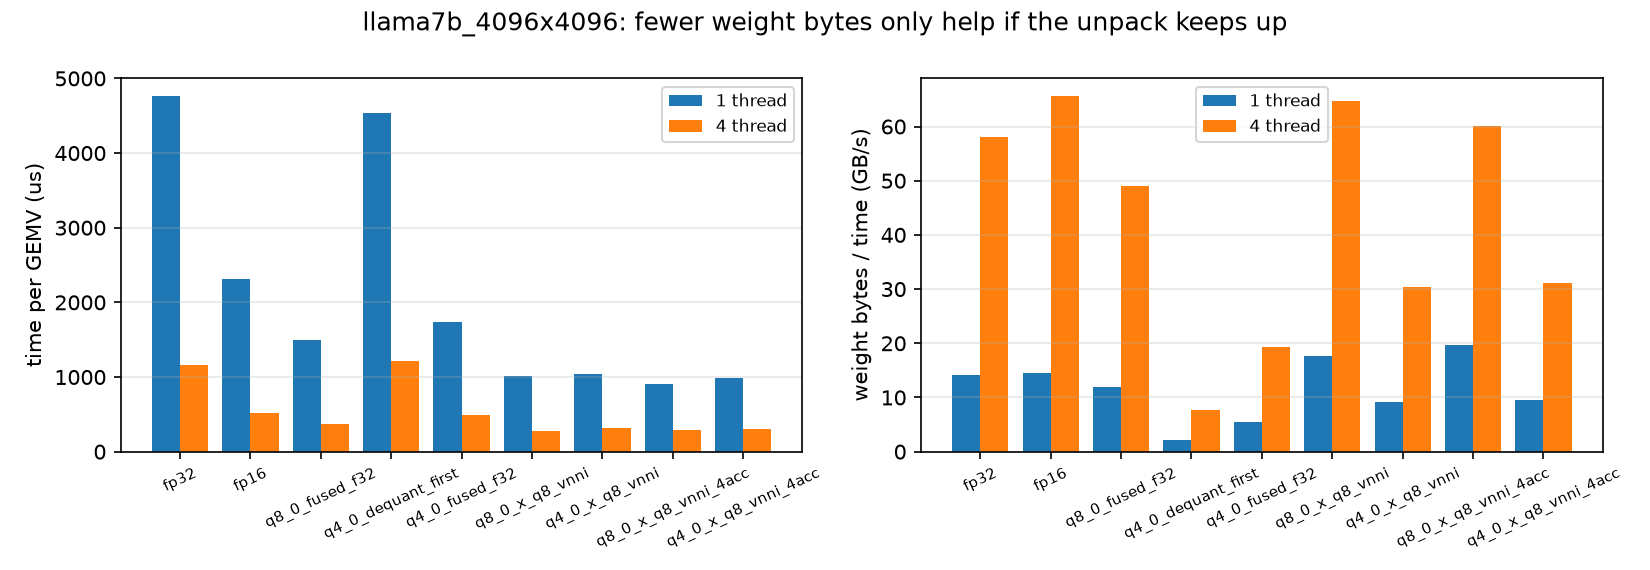
\includegraphics[width=\linewidth]{gemv_bench.png}
\caption{本机（Ice Lake 4 核 VM），Llama-7B 形状 $4096^2$。左：每次 GEMV 的中位时间；右：权重字节 ÷ 时间。蓝色 1 线程，橙色 4 线程。}\label{fig:gemv-local}
\end{figure}

\Cref{fig:gemv-local} 左图里最显眼的是两根高柱：fp32 与“Q4\_0 先反量化”几乎一样高（4763 与 4541 µs），读的字节却差 7 倍。
右图把同样的数据换成 GB/s：fp32、fp16、Q8 × Q8 的 4 线程柱都在 58--66 GB/s，接近甚至超过本机 4 线程 DRAM 流式读的 48.4 GB/s；
三种 Q4 内核的柱子都矮得多——先反量化 2.1 / 7.8 GB/s，浮点融合 5.4 / 19.3，整数点积 9.1 / 30.3。Q4 的“GB/s”低并不表示它慢，而是说它每读一个字节要做的事更多：
\emph{字节少到一定程度，瓶颈就从搬字节换成了拆字节。}

\begin{table}[H]
\centering\small
\caption{本机，Llama-7B 形状 $4096\times4096$（\texttt{gemv\_bench.csv}，15 次重复中位数）。权重字节：fp32 67 MB、fp16 33.5 MB、Q8\_0 17.8 MB、Q4\_0 9.4 MB}\label{tab:gemv-local}
\begin{tabular}{lrrrrr}
\toprule
方法 & 1 线程 µs & GB/s & 4 线程 µs & GB/s & 4 线程加速比 \\
\midrule
fp32 & 4763 & 14.1 & 1156 & 58.1 & 4.12 \\
fp16 & 2312 & 14.5 & 511 & 65.6 & 4.52 \\
Q8\_0 浮点融合 & 1494 & 11.9 & 364 & 48.9 & 4.10 \\
Q4\_0 先反量化 & 4541 & 2.1 & 1214 & 7.8 & 3.74 \\
Q4\_0 浮点融合 & 1743 & 5.4 & 489 & 19.3 & 3.57 \\
Q8\_0 × Q8 VNNI & 1009 & 17.7 & 275 & 64.7 & 3.66 \\
Q4\_0 × Q8 VNNI & 1034 & 9.1 & 311 & 30.3 & 3.32 \\
Q8\_0 × Q8 VNNI，4 累加器 & 903 & 19.8 & 297 & 60.0 & 3.04 \\
Q4\_0 × Q8 VNNI，4 累加器 & 990 & 9.5 & 303 & 31.1 & 3.27 \\
\bottomrule
\end{tabular}
\end{table}

\subsection{融合是前提，整数点积是关键}

三种 Q4 内核读完全相同的字节，单线程时间却是 4541、1743、1034 µs：
\begin{itemize}
  \item \textbf{先反量化}只比 fp32 快 5\%。每行先把 4096 个 fp32 写进缓冲再读回来做点积，相当于在 Q4 的 9.4 MB 之外又读写了一遍 fp32 的量；
        它的 4 线程 GB/s（7.8）是所有方法里最低的。这正是“先把权重反量化，再调用现成的 BLAS”的朴素移植会得到的结果。
  \item \textbf{浮点融合}快 2.6 倍：解包在寄存器里完成，不再写回内存；但每个权重都要走 u8 $\to$ int32 $\to$ fp32 $\to$ 减 8 $\to$ FMA。
  \item \textbf{整数点积}再快 1.7 倍（1743 / 1034）：块内 32 个乘加压成一条 \texttt{dpbusd}，每块只做一次浮点乘。对 fp32 快 4.6 倍，对 fp16 快 2.2 倍（2312 / 1034）。
\end{itemize}
同样的规律在 Q8 上也成立：Q8\_0 浮点融合 1494 µs，Q8 × Q8 VNNI 1009 µs，快 1.48 倍。

\begin{findingbox}[：Q4 单线程只兑现了字节比的 65\%]
fp32 / Q4\_0 的字节比是 $32/4.5 = 7.1$，实测时间比 $4763/1034 = 4.6$，即 65\%。换算成两个利用率：$2\times4096^2 / 1034\,\text{µs} = 32$ GOP/s，只有本机单线程 VNNI 峰值 396 的 8\%；
9.1 GB/s 只有单线程 DRAM 读 13.4 的 68\%。\emph{两个都没吃满}，说明瓶颈既不是 ALU 也不是带宽，而是每块固定的指令序列。
\end{findingbox}

\subsection{Q4 为什么追不上 Q8：否定“依赖链”假设}

Q4 × Q8 读 9.4 MB，Q8 × Q8 读 17.8 MB，单线程却是 1034 对 1009 µs，4 线程 311 对 275 µs——Q8 反而更快。
第一个假设是 FMA 累加链：一个累加器时每块的 FMA 要等上一块（延迟 4 拍）。4 累加器版在同一次运行里计时，结果如下：

\begin{table}[H]
\centering\small
\caption{四个独立累加器的效果，$4096^2$，本机}\label{tab:4acc}
\begin{tabular}{lrrr}
\toprule
 & 1 个累加器 & 4 个累加器 & 变化 \\
\midrule
Q4 × Q8，1 线程 & 1034 µs & 990 µs & $-4\%$ \\
Q8 × Q8，1 线程 & 1009 µs & 903 µs & $-11\%$ \\
Q4 × Q8，4 线程 & 311 µs & 303 µs & $-3\%$ \\
Q8 × Q8，4 线程 & 275 µs & 297 µs & $+8\%$ \\
Q4 每块耗时（1 线程） & 1.97 ns & 1.89 ns & 按 2.42 GHz 约 4.8 / 4.6 拍 \\
\bottomrule
\end{tabular}
\end{table}

每块耗时 = 单线程时间 ÷ 块数（$4096^2/32 = 524{,}288$ 块）。去掉依赖链之后 Q4 每块仍要约 4.6 拍，只快 4\%，假设被否定：
瓶颈是每块的\emph{指令吞吐}，不是依赖。按 µop 数估算，拼接、广播、fp16 转换集中在 shuffle 端口（Ice Lake 的 port 5），每块 4--5 个，与 4.6 拍同量级；
但虚拟机里没有性能计数器，这只是估算。Q8 × Q8 不用拆半字节，每块 µop 更少，原来更接近延迟链，所以单线程多累加器有 11\% 的收益；
4 线程时它已经受带宽限，多累加器反而慢 8\%。

4 线程加速比（\cref{tab:gemv-local} 最后一列）给出同一个结论：fp32 4.12 倍、Q8 × Q8 3.66 倍、Q4 × Q8 3.32 倍。Q4 的扩展最差，因为它的瓶颈是每核的指令吞吐，
加核只是把同一段指令序列复制到更多核上，而 fp32 的瓶颈是共享的带宽，单线程远没吃满它（13.4 对 48.4 GB/s，E2）。

\subsection{Q8 的 64.7 GB/s 是缓存给的}

Q8 × Q8 4 线程测到 64.7 GB/s、fp16 65.6 GB/s，都超过本机 4 线程 DRAM 流式读的 48.4 GB/s；单线程 Q8 × Q8 17.7 GB/s 也超过单核只读的 13.4。
这不是测错：同一个 17.8 MB 的矩阵被反复调用，有一部分留在 L3 里。真实的 7B 模型权重是 GB 级，每个 token 都从 DRAM 流过，这部分缓存收益不存在。
所以“4 线程时 Q8 更快”只在矩阵能部分驻留缓存时成立（\cref{sec:res-bound} 给出整模型的推算）。

\subsection{两次运行之间的漂移本身就是证据}

上一次空闲运行里 fp32 4447、Q8 × Q8 1235、Q4 × Q8 1005 µs，这一次 4763、1009、1034 µs。Q8 两次差 18\%，Q4 只差 3\%。
受带宽和缓存状态影响的内核会在两次运行之间漂移，受指令限的内核几乎不动——这是没有计数器时区分两类瓶颈的一个可用观测。
表中只用这一次运行，所有方法在同一次运行里计时，所以方法之间的比值比绝对值更可靠。

\subsection{其他三个形状}

\begin{table}[H]
\centering\small
\caption{本机四个形状，1 线程 / 4 线程 µs（\texttt{summary.json}）}\label{tab:shapes-local}
\begin{tabular}{lrrrrr}
\toprule
形状（行 × 列） & fp32 权重 & fp32 & fp16 & Q8 × Q8 & Q4 × Q8 \\
\midrule
GPT-2 MLP 3072×768 & 9.4 MB & 250.7 / 86.4 & 211.1 / 57.3 & 140.0 / 44.6 & 150.7 / 47.1 \\
Llama-1B $2048^2$ & 16.8 MB & 508.3 / 149.1 & 371.3 / 108.8 & 229.7 / 83.2 & 266.5 / 90.7 \\
Llama-1B MLP 8192×2048 & 67 MB & 4522.7 / 1115.0 & 2212.0 / 526.9 & 1083.9 / 339.0 & 1037.8 / 324.8 \\
Llama-7B $4096^2$ & 67 MB & 4763 / 1156 & 2312 / 511 & 1009 / 275 & 1034 / 311 \\
\bottomrule
\end{tabular}
\end{table}

小矩阵全部在缓存里：GPT-2 MLP 的 fp32 4 线程 109.2 GB/s，Llama-1B $2048^2$ 112.5 GB/s，是 DRAM 流式读的 2.3 倍。
在这两个形状上，Q4 × Q8 对 fp32 单线程只快 1.66 倍（250.7 / 150.7）和 1.91 倍（508.3 / 266.5）；到 67 MB 的两个形状才拉开到 4.36 倍（8192×2048）与 4.6 倍（$4096^2$）。
\emph{Q4 的优势只在 fp32 放不进缓存、真正去读 DRAM 时出现}，这与“解码是带宽问题”一致：工作集在缓存里时，减字节就不是主要矛盾。
8192×2048 与 $4096^2$ 元素数相同，Q4 × Q8 时间几乎一样（1038 对 1034 µs），也说明它的时间由块数决定，而不是由矩阵形状决定。

\begin{iqbox}{Q4 内核的瓶颈怎么定位？没有 perf 怎么办？}
三步。第一，算两个利用率：GOP/s 对 VNNI 峰值（8\%），GB/s 对 DRAM（68\%），两个都不满，说明是指令序列本身。
第二，找一个“只去掉一项开销”的对照：Q8 × Q8 不拆半字节，单线程 17.7 GB/s（含部分 L3 命中），能更接近带宽，所以拆半字节和每块开销是嫌疑。
第三，排除依赖链：4 个独立累加器只快 4\%，所以不是延迟而是每块的指令吞吐。再补一个旁证：两次运行之间 Q4 只漂 3\%、Q8 漂 18\%，指令受限的内核对缓存状态不敏感。
下一步优化是减少每块的 shuffle µop：一次处理两行（共享 $x$ 的加载、$\sum s$ 广播与 $d_x$），或用 512 位一次处理两块、把两个 scale 拼成一个向量。
常见错答：“Q4 慢是因为内存不够快”——Q4 的 9.1 GB/s 离 13.4 GB/s 还有距离，而读两倍字节的 Q8 跑得一样快。
\end{iqbox}

\section{结果二：解码上界}\label{sec:res-bound}

\begin{table}[H]
\centering\small
\caption{解码上界 tok/s（\texttt{decode\_bound.csv}，只算 Linear 权重，不含 KV cache 与激活）。最后一列用本机 $4096^2$ 上该格式内核的实测 GB/s 换算}\label{tab:bound}
\begin{tabular}{llrrrr}
\toprule
模型 & 格式 & 权重 GB & Pi 5（17.1 GB/s） & Orin Nano（68 GB/s） & 本机 4 线程 \\
\midrule
Llama-7B & fp16 & 13.48 & 1.3 & 5.0 & 4.9 \\
Llama-7B & Q8\_0 & 7.16 & 2.4 & 9.5 & 9.0 \\
Llama-7B & Q4\_0 & 3.79 & 4.5 & 17.9 & 8.0 \\
Llama-1B & Q4\_0 & 0.70 & 24.5 & 97.5 & 43.4 \\
GPT-2 124M & Q4\_0 & 0.070 & 244.7 & 974.9 & 434.5 \\
\bottomrule
\end{tabular}
\end{table}

前两列是纯粹的 \cref{eq:bound}：带宽 ÷ 字节，格式之间严格按 bpw 缩放，Q4\_0 是 fp16 的 3.56 倍。最后一列把“内核能用到的带宽”代进去：
fp16 用 fp16 内核的 65.6 GB/s，Q8\_0 用 Q8 × Q8 的 64.7 GB/s，Q4\_0 用 Q4 × Q8 的 30.3 GB/s。于是本机 4 线程上 Q8\_0（9.0 tok/s）反而高于 Q4\_0（8.0）。

但 fp16 与 Q8 的那两个 GB/s 含 L3 命中，对 GB 级的整模型偏乐观。按 DRAM 流式 48.4 GB/s 封顶：
\begin{equation}
\text{Q8\_0}:\ \frac{7.16\ \text{GB}}{48.4\ \text{GB/s}} = 148\ \text{ms/token} \Rightarrow 6.8\ \text{tok/s};\qquad
\text{Q4\_0}:\ \frac{3.79\ \text{GB}}{30.3\ \text{GB/s}} = 125\ \text{ms/token} \Rightarrow 8.0\ \text{tok/s}.
\end{equation}
Q4 的 30.3 GB/s 低于 DRAM 上限，不受封顶影响；Q8 被封顶后降到 6.8 tok/s，\emph{结论反转回 Q4 更快}。
本机没有跑完整 7B 模型，这一段是推算；服务器上的端到端检验见 \cref{sec:server-e2e}。

\begin{iqbox}{一个 7B 模型在手机上能跑多快？}
用 E25。Llama-7B Q4\_0 是 $6.74\times10^9 \times 4.5/8 = 3.79$ GB（不是 3.37 GB：每 32 个权重还有一个 fp16 scale）。手机 LPDDR5 的有效带宽按 30--50 GB/s 算，上界 8--13 tok/s；
Pi 5 的 17.1 GB/s 只有 4.5 tok/s。实际还要乘一个内核效率：本机单线程 Q4 × Q8 只拿到 DRAM 读的 68\%，而且这个上界不含 KV cache、lm\_head（对 GPT-2 这类共享嵌入的小模型很可观）与调度开销。
追问“那换 Q8 呢”：要看内核在哪个区间——如果 Q4 内核指令受限而 Q8 内核带宽受限，两者可能一样快；本机 4 线程的单层数字甚至是 Q8 更快，但那是缓存给的。
\end{iqbox}

\section{结果三：GPT-2 困惑度}\label{sec:res-ppl}

\begin{table}[H]
\centering\small
\caption{GPT-2 124M，wikitext-2 全部 280 个 1024 token 窗口（\texttt{gpt2\_ppl.csv}、\texttt{gpt2\_layer\_sqnr.csv}）}\label{tab:ppl}
\begin{tabular}{lrrrrr}
\toprule
格式 & bit/权重 & 困惑度 & 相对 fp32 & 层平均 SQNR dB & 层 SQNR 范围 dB \\
\midrule
fp32 & 32 & 29.951 & -- & -- & -- \\
Q8\_0 & 8.5 & 29.953 & $+0.007\%$ & 45.08 & 43.44--45.99 \\
Q4\_1 & 5.0 & 32.15 & $+7.3\%$ & 21.96 & 21.18--22.52 \\
Q4\_0 & 4.5 & 31.88 & $+6.4\%$ & 21.03 & 20.25--21.83 \\
\midrule
\multicolumn{6}{l}{\footnotesize mlsys-infra compiler-compression，同一协议：fp16 29.96，W4 g128 RTN 33.27，W4 g128 GPTQ 31.20} \\
\bottomrule
\end{tabular}
\end{table}

\paragraph{协议对齐。}fp32 的 29.951 与 mlsys-infra 的 fp16 29.96 一致，说明两边自己写的前向与评测协议对齐，后面可以把两个仓库的数字放在一张表里比较。

\paragraph{Q8\_0 无损。}困惑度只差 0.002（$+0.007\%$），层平均 SQNR 45 dB。端侧部署时 Q8\_0 可以视为与 fp32 等价。

\paragraph{SQNR 的 6 dB/bit 定律。}Q8\_0 与 Q4\_0 的层平均 SQNR 差 $45.08 - 21.03 = 24.04$ dB，与 E27 预测的 $6.02 \times 4 = 24.1$ dB 几乎相同。
逐层看，三种格式 SQNR 最低的都是第 0 层的 \texttt{mlp.c\_proj}（43.44 / 21.18 / 20.25 dB），最高的都是第 11 层的 \texttt{attn.c\_proj}（45.99 / 22.52 / 21.83 dB）；
而且在三种格式、全部 12 层里，\texttt{mlp.c\_proj} 都是该层四个 Linear 中 SQNR 最低的，说明 SQNR 的差异主要由层内权重分布（E27 的常数 $C$）决定，而不是由格式决定。

\paragraph{Q4\_0 g32 与 GPTQ g128 的位置。}本仓库的 Q4\_0 是格式 + RTN（最近舍入），每 32 个一组，31.88；mlsys-infra 同协议的 W4 g128 RTN 33.27，GPTQ g128 31.20。
分组从 128 缩到 32 抵掉了 RTN 与 GPTQ 之间约三分之二的差距（33.27 $\to$ 31.88，GPTQ 是 31.20），代价是每权重多 $0.5 - 0.125 = 0.375$ bit。

\begin{findingbox}[：SQNR 高不等于困惑度低]
Q4\_1 每块多存一个 fp16 最小值（5.0 对 4.5 bit），层平均 SQNR 高 0.93 dB（21.96 对 21.03），困惑度却\emph{更差}（32.15 对 31.88）。
一个可能的解释是 Q4\_0 让每块最大幅值元素精确无误差（\cref{eq:q40}），而 Q4\_1 的零点不精确；LLM 权重里少数大幅值元素对输出的贡献不成比例，均值 SQNR 低估了它们。
这是假设：本 lab 没有做“只保护最大元素”的消融，也没有计算两种格式困惑度差的置信区间（同一组 280 个窗口，成对差 0.27）。
可以确定的只是：选格式要看困惑度（或对 fp16 的 KL 散度），不能只看 SQNR。
\end{findingbox}

\begin{iqbox}{为什么块大小是 32？为什么 llama.cpp 要把激活也量化成 Q8？}
块大小是精度与 scale 开销的折中：一个 fp16 scale 摊到 32 个权重是 0.5 bit/权重，块越小越准、开销越大。g128 时开销只有 0.125 bit，
但 GPT-2 上 RTN 困惑度从 g32 的 31.88 升到 g128 的 33.27（mlsys-infra），需要 GPTQ 这类误差补偿才能拉回 31.20。
激活量化成 Q8 是为了块内能用整数点积（x86 VNNI、ARM \texttt{sdot}）：每 32 个乘加只做一次浮点乘。激活只有一个向量，每次调用量化一次、所有输出行共用，几乎不增加字节；
测试也确认 Q4 × Q8 的总误差不超过只量化权重的 1.1 倍。为什么不 int4 × int4？激活有离群值，4 bit 不够；而且解码是带宽问题，激活到 8 bit 已经不占带宽。
\end{iqbox}

\section{CPU 本机与服务器对照}\label{sec:server}

\begin{figure}[H]
\centering
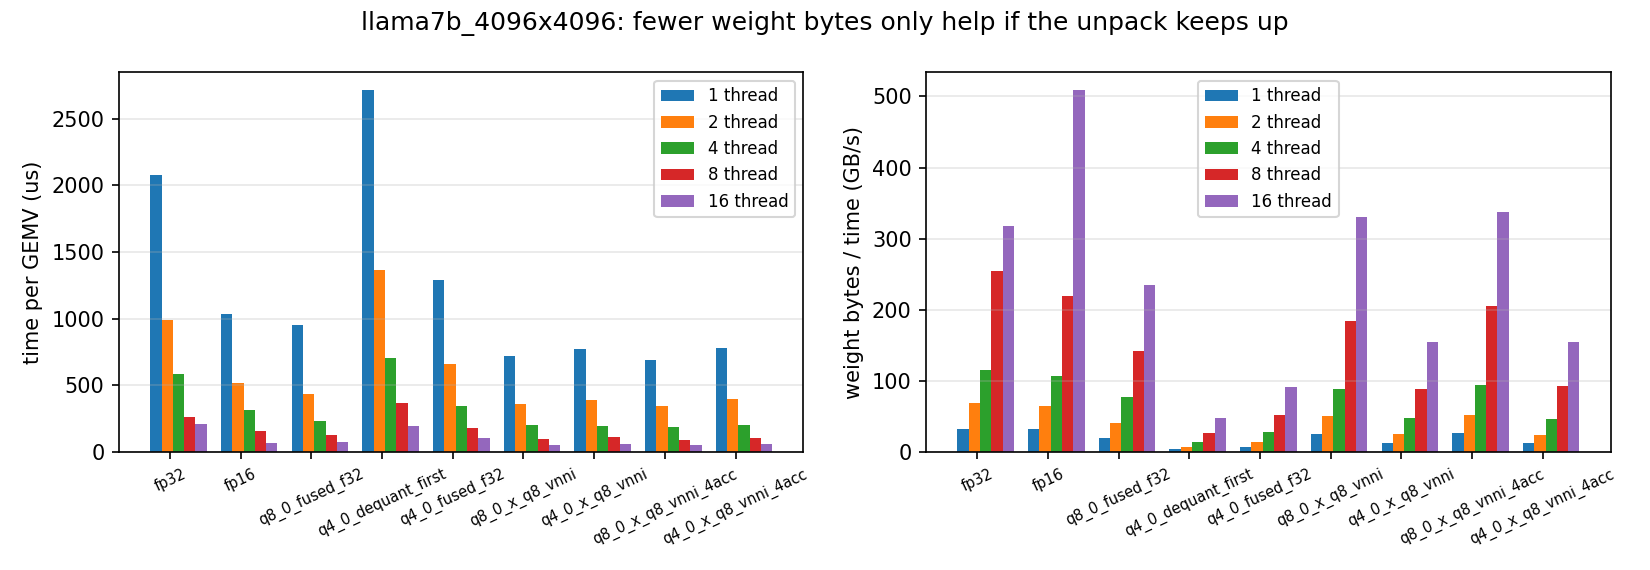
\includegraphics[width=\linewidth]{xeon8470q/gemv_bench.png}
\caption{Xeon 8470Q，Llama-7B 形状 $4096^2$，1 / 2 / 4 / 8 / 16 线程。左：每次 GEMV 的中位时间；右：权重字节 ÷ 时间。}\label{fig:gemv-xeon}
\end{figure}

\Cref{fig:gemv-xeon} 与 \cref{fig:gemv-local} 是同一张图在服务器上的版本，多了 2、8、16 线程。右图里紫色的 16 线程柱分成两组：
fp32 318、fp16 508、Q8 × Q8 330、Q8 × Q8 4 累加器 338 GB/s，远超 16 线程 DRAM 读的 193.5 GB/s——$4096^2$ 的 fp16 只有 33.5 MB、Q8 17.8 MB，整个装进 105 MB 的 L3，测的是片上缓存；
而 Q4 × Q8 的 16 线程柱只有 154 GB/s，Q4 浮点融合 91.5，先反量化 48.1。Q4 的工作集更小、更容易驻留缓存，GB/s 却更低——它与内存无关，被指令限住。
左图的单线程（蓝色）一组也重复了本机的形状：先反量化最高（2712 µs），fp32 次之（2075 µs），Q8 × Q8（719）与 Q4 × Q8（768）几乎一样矮。

\subsection{单线程：服务器只快 1.3--2.3 倍，而且快在缓存上}

\begin{table}[H]
\centering\small
\caption{$4096^2$ 单线程，本机对服务器（µs）}\label{tab:vm-vs-xeon}
\begin{tabular}{lrrr}
\toprule
方法 & 本机 VM & Xeon 8470Q & 比值 \\
\midrule
fp32 & 4763 & 2075 & 2.30 \\
fp16 & 2312 & 1033 & 2.24 \\
Q8\_0 浮点融合 & 1494 & 949 & 1.57 \\
Q4\_0 先反量化 & 4541 & 2712 & 1.67 \\
Q4\_0 浮点融合 & 1743 & 1287 & 1.35 \\
Q8\_0 × Q8 VNNI & 1009 & 719 & 1.40 \\
Q4\_0 × Q8 VNNI & 1034 & 768 & 1.35 \\
Q8\_0 × Q8 VNNI，4 累加器 & 903 & 689 & 1.31 \\
Q4\_0 × Q8 VNNI，4 累加器 & 990 & 783 & 1.26 \\
\bottomrule
\end{tabular}
\end{table}

比值分成两组：读字节多的 fp32 / fp16 快 2.2--2.3 倍，指令受限的 Q4 / Q8 整数内核只快 1.26--1.40 倍。
服务器单核 DRAM 读只比本机高 30\%（17.5 对 13.4 GB/s），所以 fp32 的 2.3 倍不是来自 DRAM，而是来自更大的 L2/L3：67 MB 的 fp32 矩阵在服务器上有更大比例留在 105 MB 的 L3 里。
整数内核的 1.3 倍与两台机器的单核频率比同量级（服务器报告由 fp32 峰值反推单核睿频 3.6 GHz，M08 笔记按 2.42 GHz 估算本机拍数，比值约 1.49），这是“指令受限的内核只随频率变快”的旁证。
4 累加器版在服务器单线程上几乎没有收益：$4096^2$ 上 Q8 快 4\%（719 $\to$ 689 µs），Q4 慢 2\%（768 $\to$ 783 µs）；11008×4096 上两者都变慢（Q8 1947 $\to$ 2036，Q4 2057 $\to$ 2121 µs），与本机的“多累加器不是答案”一致。

\subsection{Llama-7B MLP 形状 11008×4096：1--16 线程}

为了让 fp32 的工作集超过 105 MB 的 L3，服务器上新增了 11008×4096 形状（fp32 180 MB、fp16 90 MB、Q8\_0 48 MB、Q4\_0 25 MB）：

\begin{table}[H]
\centering\small
\caption{Xeon 8470Q，11008×4096（µs，\texttt{xeon8470q/summary.json}）}\label{tab:xeon-mlp}
\begin{tabular}{lrrrrrrr}
\toprule
方法 & 1 线程 & 2 线程 & 4 线程 & 8 线程 & 16 线程 & \makecell{16 线程\\GB/s} & \makecell{1$\to$16\\加速比} \\
\midrule
fp32 & 9580 & 4724 & 2545 & 1273 & 660 & 273 & 14.5 \\
fp16 & 4978 & 2111 & 1035 & 490 & 297 & 304 & 16.8 \\
Q8\_0 浮点融合 & 2400 & 1195 & 648 & 338 & 198 & 242 & 12.1 \\
Q4\_0 先反量化 & 7315 & 3672 & 1852 & 944 & 523 & 48 & 14.0 \\
Q4\_0 浮点融合 & 3545 & 1785 & 903 & 462 & 281 & 90 & 12.6 \\
Q8\_0 × Q8 VNNI & 1947 & 967 & 525 & 261 & 154 & 311 & 12.6 \\
Q4\_0 × Q8 VNNI & 2057 & 1012 & 523 & 274 & 158 & 161 & 13.0 \\
Q8\_0 × Q8 VNNI，4 累加器 & 2036 & 904 & 516 & 250 & 144 & 332 & 14.1 \\
\bottomrule
\end{tabular}
\end{table}

\begin{findingbox}[：Q4 在 CPU 上是指令受限的，加线程也不改变]
1、4、16 线程下 Q4 × Q8 与 Q8 × Q8 的时间比是 1.06、1.00、1.02，都相差不到 6\%：Q4 只读一半字节，却没有更快。
16 线程时 Q4 × Q8 只有 161 GB/s，离 L3 带宽还远（Q8 × Q8 在同一形状上到 311 GB/s）；25 MB 的 Q4 权重整个装得下 105 MB 的 L3，测的本来就是 L3 而不是 DRAM，它仍然慢，
只能是每块的解包指令。这条结论与本机在 4 核上的观测一致，属于\emph{结构性}结论：换机器只改常数，不改排序。
\end{findingbox}

fp32 的 16 线程 273 GB/s 超过 DRAM 只读的 193.5 GB/s，说明 180 MB 里仍有一大块留在 L3（逐次调用间不被冲掉）；fp16 的 1$\to$16 加速比 16.8 倍超线性，
也是同一个缓存效应——单线程时 90 MB 的 fp16 大部分从 DRAM 来，16 线程时更多的私有 L2 与共享 L3 一起把它留在片上（这一解释是推断，没有计数器验证）。
单线程一列里 fp32 18.8 GB/s，略高于单核 DRAM 读的 17.5，与“180 MB 大部分从 DRAM 来”相符；Q8 × Q8 单线程 24.6 GB/s 则明显来自 L3。

\subsection{服务器上的解码推算与 llama.cpp 端到端}\label{sec:server-e2e}

\nolinkurl{xeon8470q/decode_bound.csv} 按服务器 $4096^2$ 上各内核的实测 GB/s 换算 Llama-7B 的上界：16 线程 fp16 37.7、Q8\_0 46.1、Q4\_0 40.7 tok/s；
单线程 2.41、3.46、3.24 tok/s。和本机一样，fp16 与 Q8 的 GB/s 含缓存命中。按 16 线程 DRAM 读 193.5 GB/s 封顶（与 \cref{sec:res-bound} 同样的推算）：
fp16 $193.5/13.48 = 14.4$，Q8\_0 $193.5/7.16 = 27.0$；Q4\_0 的 154 GB/s 本来就低于 DRAM，仍为 40.7。排序是 Q4\_0 $>$ Q8\_0 $>$ fp16。

llama-cpp-7b 报告在同一台 Xeon 上用 llama.cpp 跑 Qwen2.5-7B（7.6B 参数，与 Llama-7B 不是同一个模型），16 线程实测 F16 13.4、Q8\_0 22.0、Q4\_0 37.4 tok/s。
两个模型大小接近，排序与上面的封顶推算一致：\emph{整模型流式读 DRAM 时，Q4 确实比 Q8 快}，单层 GEMV 里“Q8 与 Q4 持平”的结论不能外推到整模型。
还有两个对照值得一提：llama.cpp 单线程 Q4\_0 解码读到 16.3 GB/s（单核 DRAM 读的 93\%），而本 lab 的 Q4 × Q8 单线程在服务器上只有 12.3 GB/s——llama.cpp 的 x86 内核有多块并行等优化；
llama.cpp 关闭 AMX 重排时 Q4\_0 16 线程只有 109 GB/s，比 Q8\_0（127 GB/s）还低，“每字节要做的解包更多，先撞上指令瓶颈”，与本 lab 自写 Q4 内核的问题相同。

\begin{iqbox}{4 线程时 Q8 更快，那端侧应该部署 Q8 吗？}
先看矩阵是否驻留缓存。本机 $4096^2$ 的 Q8 测到 64.7 GB/s，超过 DRAM 流式 48.4 GB/s，说明有 L3 命中。整模型 GB 级权重每个 token 都从 DRAM 流过：
Q8 被 DRAM 限在约 6.8 tok/s，Q4 在 30.3 GB/s 时还没碰到 DRAM 上限，约 8.0 tok/s，结论反转。服务器上 llama.cpp 端到端的 Q4\_0 37.4 对 Q8\_0 22.0 tok/s 证实了这个方向。
所以要用\emph{工作集大于末级缓存}的形状测（服务器上的 11008×4096 就是为此加的），或者直接测端到端；单层重复调用的 GEMV 只能定位内核瓶颈，不能决定格式。
\end{iqbox}

\section{GPU：Triton 融合反量化与解码预测}\label{sec:gpu}

\subsection{单层 GEMV：融合之后只剩搬字节}

\begin{table}[H]
\centering\small
\caption{RTX 6000D，M = 1，L2 冷，CUDA graph（µs，\texttt{gpu/gemv\_gpu.csv}）；“eager”列为 Triton Q4\_0 的 eager 下发}\label{tab:gpu-gemv}
\begin{tabular}{lrrrrrrr}
\toprule
形状（N×K） & \makecell{cuBLAS\\fp16} & \makecell{Triton\\fp16} & \makecell{Triton\\Q8\_0} & \makecell{Triton\\Q4\_0} & \makecell{Q4\_0\\eager} & \makecell{Q4\_0 反量化\\+ cuBLAS} & \makecell{W4A16 TC\\M=1} \\
\midrule
Llama $4096\times4096$ & 28.5 & 26.8 & 15.7 & 10.3 & 23.8 & 276 & 41.0 \\
Llama 11008×4096 & 69.7 & 68.5 & 38.5 & 20.7 & 23.3 & 1076 & 53.9 \\
Qwen q/o 3584×3584 & 24.2 & 20.7 & 11.8 & 7.5 & 23.8 & 172 & 36.1 \\
Qwen k/v 512×3584 & 5.7 & 4.8 & 4.0 & 3.7 & 24.8 & 28.3 & 35.9 \\
Qwen gate/up 18944×3584 & 110.0 & 103.2 & 56.7 & 31.4 & 32.0 & 1774 & 50.5 \\
Qwen down 3584×18944 & 106.9 & 103.4 & 58.6 & 32.4 & 33.1 & 1786 & 196.8 \\
Qwen lm\_head 152064×3584 & 838 & 811 & 433 & 231 & 232 & 15489 & 351 \\
\bottomrule
\end{tabular}
\end{table}

\begin{findingbox}[：GPU 上量化 GEMV 的时间严格按字节缩放]
lm\_head（1.09 GB fp16 权重）上 Triton fp16 1344、Q8\_0 1337、Q4\_0 1327 GB/s，都在 4 GB 顺序读 1333 GB/s 的 $\pm1\%$ 内；Q4\_0 是实测读带宽的 99.5\%。
时间比 cuBLAS fp16 / Triton Q4\_0 $= 838/231 = 3.63$，与 16 bit / 4.5 bit $= 3.56$ 的字节比几乎相同。GPU 每字节可用的 ALU 足以藏住拆半字节与乘 scale——
与 CPU 上 Q4 被指令吞吐卡住（\cref{sec:server}）正好相反。同样的 Q4\_0 格式，在 CPU 上是指令问题，在 GPU 上是带宽问题。
\end{findingbox}

\begin{figure}[H]
\centering
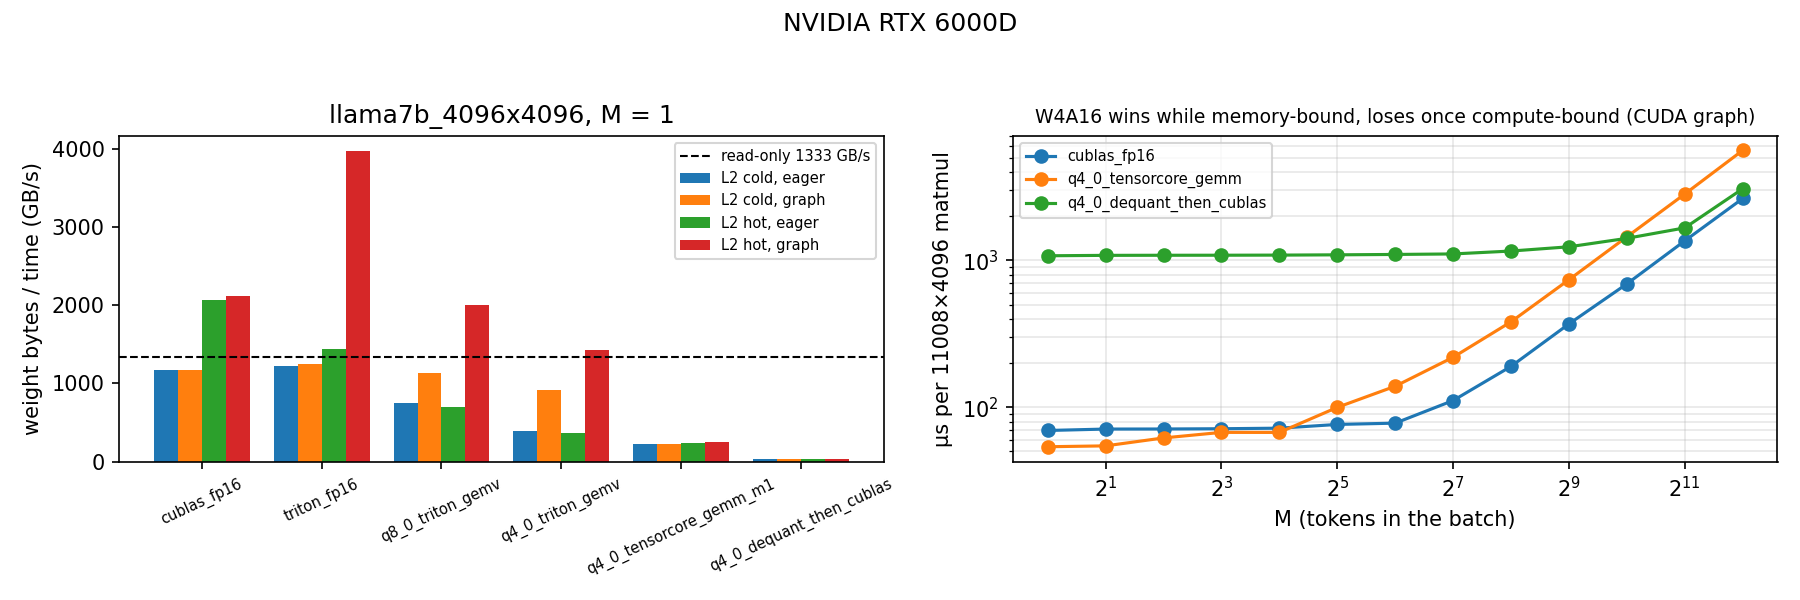
\includegraphics[width=\linewidth]{gemv_gpu.png}
\caption{RTX 6000D。左：Llama-7B $4096^2$、M = 1 时每种方法的权重字节 ÷ 时间，四种组合为 L2 冷 / 热 × eager / graph，虚线为 4 GB 只读 1333 GB/s；右：11008×4096 的 batch 扫描（CUDA graph，对数坐标）。}\label{fig:gemv-gpu}
\end{figure}

\Cref{fig:gemv-gpu} 左图在 $4096^2$ 这一个形状上展示计时协议有多重要。同一个 Triton fp16 kernel：L2 冷 graph 1250 GB/s（在虚线下方），L2 热 graph 3975 GB/s（红柱，虚线的 3 倍）——
33.5 MB 的权重整个驻留 112 MB 的 L2，测到的是 L2 带宽。Q8\_0 与 Q4\_0 的热 graph 柱也有 2009 与 1431 GB/s。而 7B 整模型每 token 要读 4--14 GB，必然来自 DRAM，所以\emph{只有 L2 冷的数字能用来预测解码}。
同一张图里 eager 与 graph 的差别也清楚：Q4\_0 冷 eager 只有 396 GB/s（23.8 µs，基本就是下发开销），冷 graph 913 GB/s（10.3 µs）；Q8\_0 从 746 升到 1139 GB/s。
fp16 的 eager 与 graph 几乎一样（26.8 对 27.5 µs），因为 33.5 MB 要读 25 µs 左右，本来就比下发地板长。最右边两组（W4A16 TC 约 230 GB/s，先反量化 + cuBLAS 约 34 GB/s）无论冷热都贴近底部。

右图是 11008×4096 上的 batch 扫描，下一小节讨论。

\begin{figure}[H]
\centering
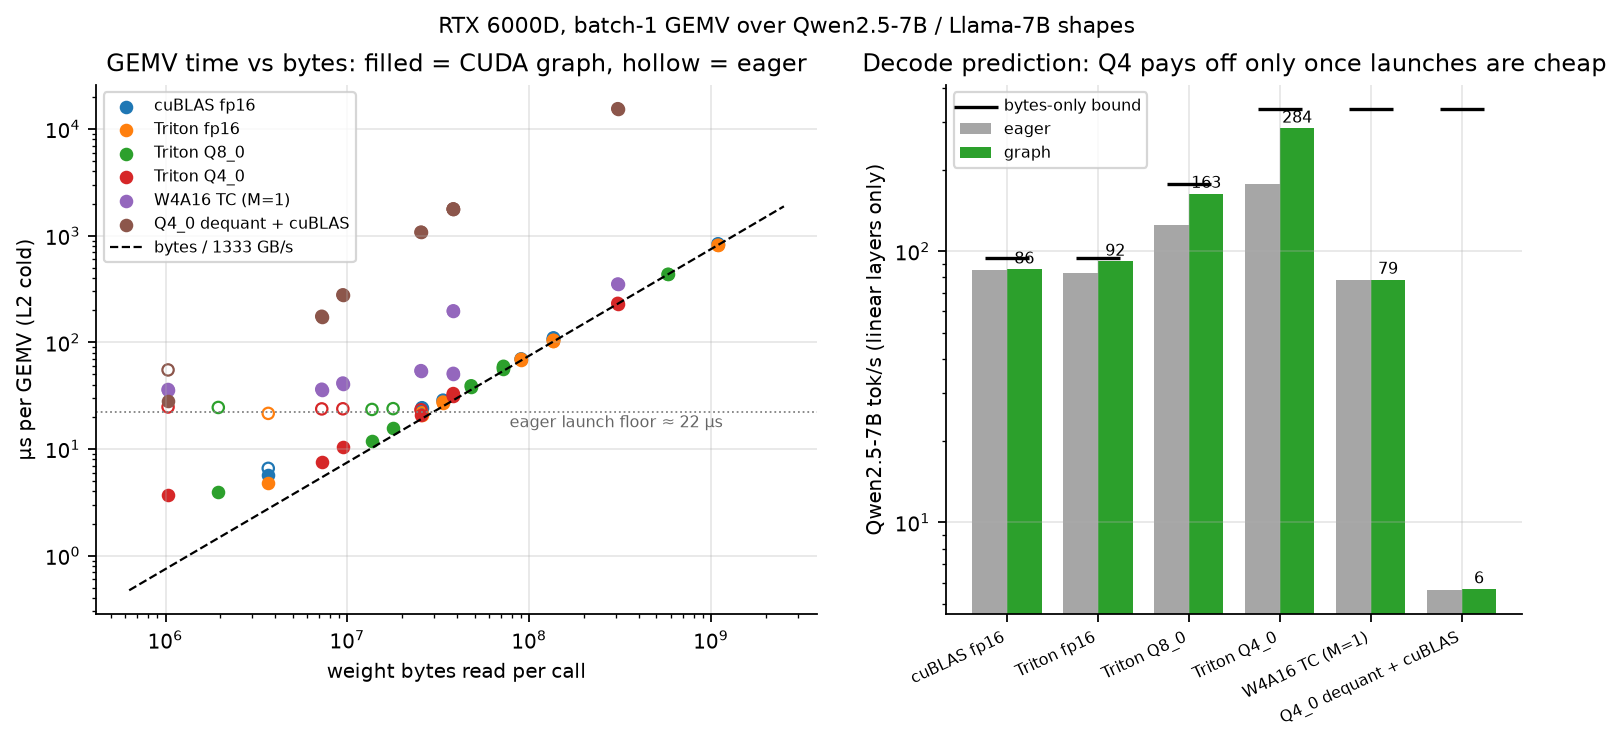
\includegraphics[width=\linewidth]{gemv_gpu_roofline.png}
\caption{RTX 6000D，Qwen2.5-7B / Llama-7B 各形状的 batch 1 GEMV。左：每次 GEMV 的时间对读取字节数（实心 = CUDA graph，空心 = eager），虚线为 bytes / 1333 GB/s，点线为约 22 µs 的 eager 下发地板；
右：把左图换算成只算 Linear 的 Qwen2.5-7B 解码 tok/s（灰 eager、绿 graph），黑横线为只算字节的上界。}\label{fig:gpu-roofline}
\end{figure}

\Cref{fig:gpu-roofline} 左图把每次 GEMV 画在“读了多少字节”上，一个点离虚线越近，越接近只受带宽限制。可以读出三个区域：
\begin{itemize}
  \item \textbf{30 MB 以上}：各融合方法的实心点（graph）都落在虚线上，与格式无关。只要融合，GPU 上的量化 GEMV 就只剩搬字节一件事。
  \item \textbf{10 MB 以下}：空心点（eager）贴着约 22 µs 的水平点线，这条线就是 Python + Triton 的下发开销，与形状无关——k/v 投影的 Q4 权重只有约 1 MB，eager 也要 24.8 µs，graph 后 3.7 µs。
        Q4 把字节压到 1/3.6，却把更多层推到了这条线下面，所以\emph{eager 模式下量化越狠、收益越少}。
  \item \textbf{离线很远的两类}：棕色点（先反量化 + cuBLAS）比虚线高一个半数量级——每次都把 fp16 权重写出再读回，比 fp16 GEMV 慢 15--70 倍（lm\_head 15489 对 811 µs）；
        紫色点（W4A16 tensor core）在大 K 时也离线很远：M = 1 时 \texttt{tl.dot} 的 16 行 tile 有 15 行是空的，down（K = 18944）上 196.8 µs，是 Triton Q4\_0 GEMV 的 6 倍。
\end{itemize}
右图把左图换算成整模型解码速度：Triton Q4\_0 graph 284 tok/s，是唯一一个 eager（176）与 graph 差距大的方法；cuBLAS fp16 与 Triton fp16 都接近上界横线（86、92），
W4A16 TC 79、先反量化 + cuBLAS 6 tok/s 远低于上界。

\subsection{解码预测}

\begin{table}[H]
\centering\small
\caption{Qwen2.5-7B 只算 Linear 的解码预测（\texttt{gpu/decode\_pred.csv}）}\label{tab:decode}
\begin{tabular}{lrrrrr}
\toprule
方法 & 权重 GB & eager tok/s & graph tok/s & graph ms/token & 占读带宽上界 \\
\midrule
cuBLAS fp16 & 14.14 & 85.1 & 85.8 & 11.66 & 91\% \\
Triton fp16 & 14.14 & 83.3 & 91.7 & 10.91 & 97\% \\
Triton Q8\_0 & 7.51 & 124.9 & 163.0 & 6.13 & 92\% \\
Triton Q4\_0 & 3.98 & 176.4 & \textbf{283.7} & 3.53 & 85\% \\
W4A16 TC（M=1） & 3.98 & 78.1 & 78.6 & 12.72 & 23\% \\
Q4\_0 反量化 + cuBLAS & 3.98 & 5.6 & 5.7 & 176.07 & 2\% \\
\bottomrule
\end{tabular}
\end{table}

上界列是 1333 GB/s ÷ 权重字节：fp16 94.3、Q8\_0 177.4、Q4\_0 335.1 tok/s。Q4 的收益只在 graph 模式下兑现：eager 时 196 个层内 Linear 每个都要付下发地板，
Q4 只比 Triton fp16 快 2.1 倍（176.4 / 83.3）；graph 后 3.1 倍（283.7 / 91.7），接近 3.56 的字节比。Q4 eager 与 graph 每 token 差 2.14 ms（5.67 对 3.53 ms），全部是下发开销。
即使在 graph 下，Q4 也只到上界的 85\%：小层（k/v 3.7 µs、q/o 7.5 µs）的固定成本占比随字节减少而上升。

\begin{iqbox}{CUDA graph 为什么能让量化解码明显变快？}
eager 模式下每个 kernel 都要经过 Python、Triton 的参数处理和驱动提交，本机约 22 µs 一次，与 kernel 大小无关。7B 模型每 token 196 次层内 Linear，
光下发就是 $196 \times 22\,\text{µs} \approx 4.3$ ms，而 Q4 权重全部读完只要 $3.98\,\text{GB} / 1333\,\text{GB/s} \approx 3$ ms——下发比搬字节还贵。
CUDA graph 把整串 kernel 一次捕获、一次提交，每个节点的开销降到几 µs（k/v 投影 3.7 µs），小层回到带宽受限。代价是形状必须固定（静态 KV cache、固定 batch），
真实推理引擎因此都用 graph 或 persistent kernel。常见错答：“量化后 kernel 更快，所以解码更快”——eager 时 Q4 的 kernel 本身更快，但 Q4 对 fp16 只快 2.1 倍。
\end{iqbox}

\subsection{batch 扫描：一过 16 就换 kernel}

\begin{table}[H]
\centering\small
\caption{batch 扫描，11008×4096，CUDA graph（µs，\texttt{gpu/batch\_sweep.csv}）}\label{tab:batch}
\begin{tabular}{rrrrl}
\toprule
M & cuBLAS fp16 & W4A16 TC & Q4 反量化 + cuBLAS & 最快 \\
\midrule
1 & 69.5 & 53.9 & 1077 & W4A16 \\
4 & 71.1 & 61.8 & 1086 & W4A16 \\
16 & 72.1 & 67.4 & 1088 & W4A16 \\
32 & 76.4 & 99.9 & 1093 & cuBLAS \\
128 & 111.2 & 219.2 & 1108 & cuBLAS \\
512 & 370.0 & 740.1 & 1240 & cuBLAS \\
1024 & 693.4 & 1450.1 & 1416 & cuBLAS（反量化版已快过 W4A16） \\
4096 & 2645.5 & 5630.6 & 3083 & cuBLAS \\
\bottomrule
\end{tabular}
\end{table}

\Cref{fig:gemv-gpu} 右图是这张表的对数坐标版本。三条曲线分成三段：
$M \le 16$ 时读权重主导，cuBLAS fp16 几乎是一条水平线（69.5--72.1 µs，读 90 MB），4 bit 权重的 W4A16 占优（53.9--67.4 µs）；
$M \ge 32$ 进入算力区，W4A16 的曲线以斜率 1 上升，我们的 kernel 只到约 65 TFLOP/s（M = 4096 时 65.6），cuBLAS 到 133--140，内层循环里的反量化开销显形；
$M \ge 1024$ 时连“先反量化再 cuBLAS”（绿色）都比 W4A16 快——反量化一次约 1 ms 的成本被 1024 行摊薄了，之后就是 cuBLAS 的 fp16 GEMM。
这正是 vLLM 等引擎对 decode 用 Marlin 类 W4A16 kernel、对 prefill 先反量化或直接用 fp16 / fp8 GEMM 的原因。

\begin{iqbox}{4 bit 量化一定让解码变快吗？}
只在“读权重”是瓶颈时成立。本 lab 测到三种不成立的情况：（1）CPU 上解包指令与点积争用向量端口，Q4 × Q8 与 Q8 × Q8 一样快（服务器 1--16 线程相差不到 6\%）；
（2）GPU 上若用 eager 逐层下发，小层被约 22 µs 的固定开销主导，字节省下来也没用（Q4 对 fp16 只快 2.1 倍）；
（3）batch 大了进入算力区，反量化变成内层循环的额外指令（M $\ge$ 32 时 W4A16 慢于 cuBLAS fp16）。
要兑现收益需要：反量化融合进 GEMV、用 CUDA graph 或 persistent kernel 消除下发开销、decode 与 prefill 用不同 kernel。
在服务端高并发下，量化的价值从“每步更快”变成“省显存、放更多 KV cache”。
\end{iqbox}

\subsection{预测与 llama.cpp 端到端的对照}\label{sec:pred-check}

本 lab 的解码预测只把单层 GEMV 时间相加，没有 attention、RMSNorm、RoPE、采样，也没有层间融合。llama-cpp-7b 报告在同一张 RTX 6000D 上用 llama.cpp（全部层 offload）跑 Qwen2.5-7B，检验了这个预测：

\begin{table}[H]
\centering\small
\caption{本 lab 的预测（196 个层内 Linear + lm\_head，CUDA graph）对 llama.cpp 端到端（llama-cpp-7b 报告）}\label{tab:pred}
\begin{tabular}{lrrrrr}
\toprule
格式 & 预测 tok/s & 实测 tok/s & 比值 & 每 token 时间差 & 加 0.45 ms 后的预测 \\
\midrule
fp16 / F16 & 91.7（10.91 ms） & 87.9（11.38 ms） & 0.96 & 0.47 ms & 88.0 \\
Q8\_0 & 163.0（6.13 ms） & 152.8（6.54 ms） & 0.94 & 0.41 ms & 151.9 \\
Q4\_0 & 283.7（3.53 ms） & 250.7（3.99 ms） & 0.88 & 0.46 ms & 251.6 \\
\bottomrule
\end{tabular}
\end{table}

\begin{findingbox}[：层时间之和只差一个常数项]
三种格式的端到端解码都比只算 Linear 的预测多 0.41--0.47 ms/token，与权重字节（14.1、7.5、4.0 GB）无关。这是 Linear 以外的每 token 固定成本：28 层的 attention、
RMSNorm、RoPE、残差、采样与 llama.cpp 的图调度。最后一列是本报告的推算：给预测加一个 0.45 ms 的常数，三种格式都落在实测的 $\pm1\%$ 以内（88.0 对 87.9、151.9 对 152.8、251.6 对 250.7）。
本 lab 的模型在结构上是对的，缺的就是这个常数；权重越小它占比越大（F16 4\%，Q4\_0 12\%），这也是比值从 0.96 降到 0.88 的原因。要让 Q4 解码更快，下一步要优化的是这 0.45 ms，而不是 GEMV kernel。
\end{findingbox}

\section{结论}\label{sec:conclusion}

\begin{findingbox}[：把“4 bit 让解码快 4 倍”拆成三个可检验的假设]
\begin{enumerate}[label=\arabic*.]
  \item \textbf{字节}：Q4\_0 是 4.5 bit/权重，不是 4；对 fp16 的字节比是 3.56 倍。本 lab 的打包器与 gguf 逐字节一致，这个数字是 llama.cpp 的真实格式。
  \item \textbf{时间正比于字节}：在 GPU 上成立——融合 kernel 在 30 MB 以上的层都落在 bytes / 1333 GB/s 上，lm\_head 的时间比 3.63 对字节比 3.56；
        在 CPU 上不成立——Q4 × Q8 与 Q8 × Q8 一样快，被每块约 4.6 拍的解包指令限住；在小矩阵（缓存内）上也不成立。
  \item \textbf{内核能兑现}：需要三个条件。融合（先反量化毫无收益）、整数点积（比浮点融合快 1.7 倍）、低下发开销（eager 时 Q4 只比 fp16 快 2.1 倍，graph 后 3.1 倍）。
\end{enumerate}
精度上 Q8\_0 无损，Q4\_0 g32 掉 6.4\% 困惑度，介于 g128 的 RTN 与 GPTQ 之间；Q4\_1 的 SQNR 更高、困惑度更差，选格式要看困惑度。
整模型上，层时间之和只差一个 0.41--0.47 ms 的常数，“减字节”的模型在 GPU 上可以直接用来估算解码速度。
\end{findingbox}

\begin{findingbox}[：哪些结论换机器不变]
\begin{itemize}
  \item 结构性：融合的必要性（先反量化对 fp32 的收益在两台机器上都不超过 1.3 倍，服务器 $4096^2$ 上甚至更慢，2712 对 2075 µs）、Q4 在 CPU 上指令受限（本机 4 核与服务器 16 核上 Q4 与 Q8 都持平）、SQNR 的 6 dB/bit。
  \item 位置性：4 线程时 Q8 比 Q4 快——取决于矩阵是否驻留缓存，整模型流式读 DRAM 时反转（服务器上 llama.cpp 的 Q4\_0 37.4 对 Q8\_0 22.0 tok/s）；
        GPU 上 Q4 的收益——取决于下发开销与层大小的比值，eager 与 graph 差 1.6 倍。
\end{itemize}
\end{findingbox}

\section{20 秒讲法}\label{sec:pitch}

解码是 GEMV，token/s 的天花板是带宽除以权重字节，Q4\_0 是 4.5 bit，把天花板抬高 3.56 倍。能不能碰到天花板取决于内核：在 CPU 上，先反量化毫无收益，整数点积单线程拿到字节比的 65\%，
而且 Q4 与读两倍字节的 Q8 一样快——它是指令受限的，加到 16 线程也一样；在 GPU 上，融合 kernel 读到实测带宽的 99.5\%，时间严格按字节缩放，但必须用 CUDA graph 去掉每层 22 µs 的下发地板。
把 196 个层的时间相加，预测 Q4 解码 284 tok/s，llama.cpp 实测 251，差的是一个与格式无关的 0.45 ms 常数。精度上 Q8 无损，Q4 掉 6\% 困惑度。

\section{不能推出的结论}\label{sec:caveats}

\begin{caveatbox}
\begin{itemize}
  \item GEMV 测的是单层、重复调用；$4096^2$ 的矩阵会部分留在 L3，不代表整模型每 token 都从 DRAM 读的情况。本机 Q8 的 64.7 GB/s、服务器 fp32 的 273 GB/s 都含缓存命中。
  \item 解码上界只算权重字节，不含 KV cache、lm\_head（GPT-2 里 38.6M 参数）、调度和采样开销；本机“Q4 比 Q8 快”的整模型结论是推算，本机没有跑完整 7B 模型。
  \item Q4\_0 与 Q4\_1 的困惑度差 0.27，没有做置信区间；“最大幅值元素精确”能否解释它只是假设，没有做消融。
  \item Pi 5 与 Orin Nano 两列是用设备表带宽算出的上界，不是实测。
  \item GPU 解码预测只把单层 GEMV 时间相加：没有 attention、RMSNorm、RoPE、采样，也没有层间融合；端到端数字来自 llama-cpp-7b 报告，且两者的引擎不同（Triton 对 llama.cpp 的 CUDA kernel）。
        “加 0.45 ms 常数后落在 $\pm1\%$ 内”是本报告对三个点的推算，不是独立的验证实验。
  \item 主机没有性能计数器权限（\texttt{ncu} 报 \texttt{ERR\_NVGPUCTRPERM}，CPU 两台都没有 perf），GPU 上“受带宽限制”、CPU 上“受指令（shuffle 端口）限制”的判断只来自墙钟时间 ÷ 字节数与对照实验，没有 DRAM 事务或端口占用率佐证。
  \item CPU 权重是合成的高斯 + 离群值矩阵，只影响计时用的数值，不影响字节与指令数；困惑度用的是真实 GPT-2 权重。
  \item 服务器与本机的编译器不同（GCC 11.4 对 MinGW g++ 13.2），跨主机比值混合了硬件与编译器两个因素；服务器 cgroup 有其他租户，16 线程的个别点可能被限流。
  \item 本 lab 只实现最基础的 Q4\_0 / Q8\_0 / Q4\_1；llama.cpp 的 x86 内核还有多块并行、K-quant（Q4\_K 等超块格式）与 imatrix，本 lab 的内核速度不代表 llama.cpp 的内核速度。
\end{itemize}
\end{caveatbox}

\section{复现}\label{sec:repro}

\begin{lstlisting}[language=bash]
cd solutions/edge-runtime/q4-gemv
python -m pytest -q tests                          # sizes, byte-exact vs gguf, C++ packer, kernel errors, GPT-2 causality
python scripts/run_experiments.py --only bench     # CPU timing on an idle machine, ~2 min
python scripts/run_experiments.py --only gpt2      # needs .data/hf/models/gpt2 and wikitext-2, ~18 min for 4 formats
python scripts/run_experiments.py --only           # rebuild summary.json and decode_bound.csv from artifacts/raw only
EDGE_THREADS=1,2,4,8,16 python scripts/run_experiments.py --only bench   # thread sweep on a many-core server

# GPU (CUDA + Triton, ~7 min, results in artifacts/raw/gpu/)
python gpu/bench_gpu.py check                      # Triton kernels vs fp32 reference
python gpu/bench_gpu.py all                        # bandwidth / gemv / sweep / decode / plot
\end{lstlisting}

GPT-2 权重和 wikitext-2 通过 hf-mirror 下载到 \nolinkurl{<repo>/.data/hf/}（可用 \texttt{EDGE\_HF\_HOME} 改路径），不入库；\texttt{--windows N} 只评测 N 个随机窗口（默认 0 = 全部 280 个）。
服务器上的结果入库时放在 \nolinkurl{artifacts/raw/xeon8470q/}，图在 \nolinkurl{artifacts/figures/xeon8470q/}。
原始数据都在 \nolinkurl{solutions/edge-runtime/q4-gemv/artifacts/raw/}，本报告的每个表都可以从那里重建。


\begin{thebibliography}{99}
\bibitem{llamacpp} G.~Gerganov et al. llama.cpp: LLM inference in C/C++. \url{https://github.com/ggml-org/llama.cpp}, 2023--2026.
\bibitem{gpt2} A.~Radford, J.~Wu, R.~Child, D.~Luan, D.~Amodei, I.~Sutskever. Language Models are Unsupervised Multitask Learners. OpenAI, 2019.
\bibitem{wikitext} S.~Merity, C.~Xiong, J.~Bradbury, R.~Socher. Pointer Sentinel Mixture Models. \emph{ICLR}, 2017.
\bibitem{triton} P.~Tillet, H.~T.~Kung, D.~Cox. Triton: An Intermediate Language and Compiler for Tiled Neural Network Computations. \emph{MAPL}, 2019.
\bibitem{gptq} E.~Frantar, S.~Ashkboos, T.~Hoefler, D.~Alistarh. GPTQ: Accurate Post-Training Quantization for Generative Pre-trained Transformers. \emph{ICLR}, 2023.
\bibitem{roofline} S.~Williams, A.~Waterman, D.~Patterson. Roofline: An Insightful Visual Performance Model for Multicore Architectures. \emph{Communications of the ACM}, 52(4), 2009.
\end{thebibliography}

\end{document}
